\documentclass[twocolumn,showpacs,preprintnumbers,amsmath,amssymb]{revtex4}

\usepackage{graphicx}  % Include figure files
\usepackage{dcolumn}   % Align table columns on decimal point
\usepackage{bm}        % bold math

\begin{document}

\preprint{APS/123-QED}

\title{Silver nanoparticle doped As$_2$S$_3$ chalcogenide
  films: A Photo-induced dissolution study }

\author{Chao Lu}
\author{Craig Arnold}
\email{cbarnold@princeton.edu}
\affiliation{Princeton University}
\date{\today}

\begin{abstract}
  Photo-induced dissolution of silver across an As$_2$S$_3$
  thin film layer is studied.
\end{abstract}

\pacs{Valid PACS appear here}    %PACS, the Physics and Astronomy Classification Scheme.
\keywords{photo-induced phenomena, silver dissolution, As$_2$S$_3$, chalcogenide films}
\maketitle

\section{\label{sec:intro}Introduction}
Chalcogenide glass material exhibit a variety of optical properties
that make them desirable for near- and mid-infrared communications and
sensing applications. We have developed silver nanoparticle doping
techniques to obtain optically sensitive chalcogenide materials, whose
response to light radiation is controllable. Such new materials hold
promise for new devices in the field of mid-IR technologies.

The diffusion of silver into chalcogenide glasses (ChG) has been
reported already more than 40 years ago by Kostyshin, but it is still
intensly studied worldwide due to the variety of its potential
applicability in areas like Mid-IR holographic volume gratings.

By doping silver nanoparticles into chalcogenide, we creates a novel
material which response to light radiation sensitively. Exposed to
visible light, either broadband source or laser, silver particles
shall react with chalcogenide matrix, and get absorbed. This structure
changes results in all kinds of physical parameters modification, such
as absorption coefficients of light, refractive index, which enables
appropriate application.

Particle doping technology, employed in preparation process, endows a
whole set of freedom to control the properties of the resulting
material. The size, shape, concentration of the particles, as well as
preparation environment like temperature and pressure, provide a
powerful parameter space to fabricate the desired material.
\section{Experiment}
\subsection{Synthesis of Silver Nanoparticles}
Materials. Ag$_2$SO$_4$ (Baker Analyzed reagent), AgNO$_3$,
(MCB), sodium citrate (Mallinckrodt, Analytical Reagent),
poly(viny1 alcohol) denoted PVA (Polysciences, hydrolysis
99.0-99.8  mol\%), were used as received.
Water was triplly distilled.
\\
Preparation of Sols. Three different kinds of Ag sols
were prepared  according to the following procedures:

(a) Ag$_2$SO$_4$ (80 mg) was dissolved in 200 mL of hot
water and then mixed with 5 g of PVA dissolved in 200
mL of hot water.  The mixture was then bubbled with H$_2$
at near boiling temperature for $3$ h.  The final volume was
adjusted to 500 mL.

(b) A solution of  $5 \times 10^{-3} M $ AgNO$_3$,  ($100$ mL) was added
portionwise to 300 mL of vigorously stirred ice-cold  $2 \times
10^{-3} M$, NaBH$_4$. A solution of  $1$\% PVA ($50$ mL) was added
during the reduction.  The mixture was then boiled for $1$ h to
decompose any excess of NaBH$_4$,.  The final volume
was adjusted to $500$ mL.

(c) AgNO$_3$,  ($90$ mg) was dissolved in $500$ mL of  H$_2$O and
brought to boiling.  A solution of  $1$\% sodium citrate ($10$
mL) was added.  The solution was kept on boiling for 1 h.
The Ag  sols  prepared  by  procedures  a  and  b  were
brownish and had absorption maximum at $400$ nm while
that prepared by procedure c was greenish yellow and had
absorption maximum at $420$ nm.

\begin{figure}[!h]
  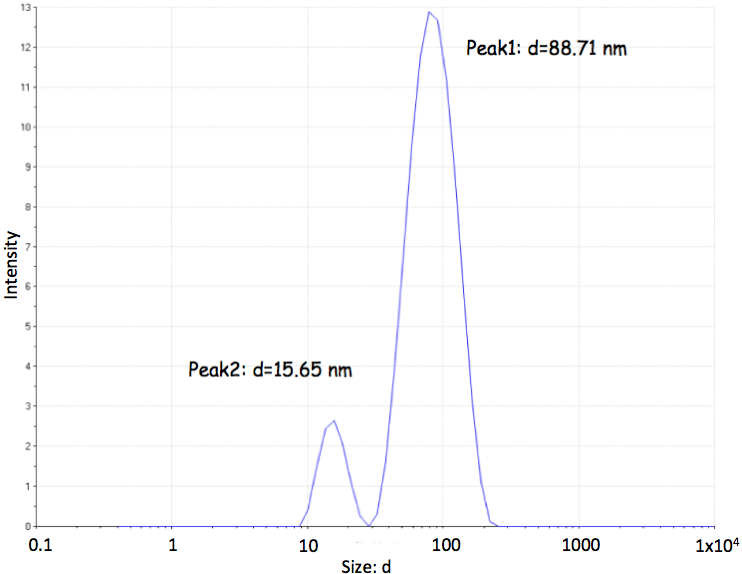
\includegraphics[width=3.25in]{figure/DLS.png}
  \caption{DLS study of the silver colloid solution}
  \label{fig:setup}
\end{figure}

\subsection{Film Exposure and Test}
\begin{figure}[!h]
  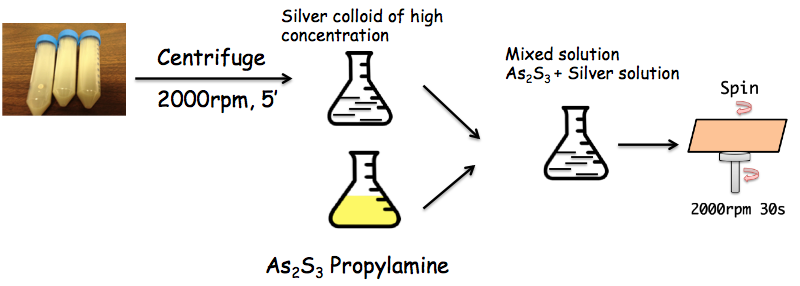
\includegraphics[width=3.25in]{figure/Film.png}
  \caption{Preparation of the film}
  \label{fig:setup}
\end{figure}

\begin{figure}[!h]
  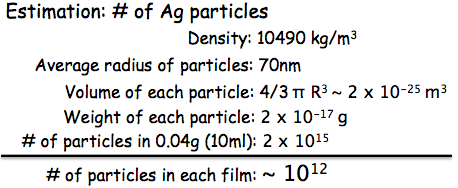
\includegraphics[width=2.75in]{figure/SilverNumber.png}
  \caption{Estimation of \# of silver particles}
  \label{fig:setup}
\end{figure}

Chalcogenide materials are first dissolved in an appropriate amine
solvent, such in arsenic sulfide in propylamine.

Silver nanoparticle of different size, shape are synthesized by
chemical reduction reactions, where species of reagents, temperature
of reaction will affect the properties of resultant particles.

Silver nanoparticles, in an appropriate concentration, are mixed into
chalcogenide solution. The solution is ready to use after an
incubation time.

Mixed silver-chalcogenide solution is spin-coated onto substrates,
like glass slides, silicon, or sodium chlorides to fabricate films for
future use. A baking process is employed thereafter to get rid of the
amine solution.


\begin{figure}[!h]
  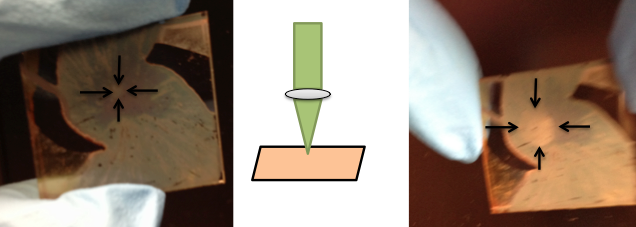
\includegraphics[width=3.25in]{figure/Exposure1.png}
  \caption{Film Illumination with Green laser ($\lambda = 532nm$)
    $50$mW $0.5$ hours in Air.}
  \label{fig:setup}
\end{figure}

\begin{figure}[!h]
  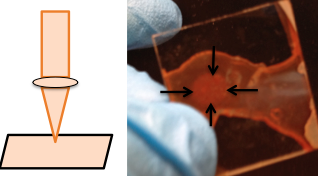
\includegraphics[width=1.75in]{figure/Exposure2.png}
  \caption{Film Illumination with Broadband $100$mW $0.5$ hours in Glovebox.}
  \label{fig:setup}
\end{figure}

\subsection{Transmission Study}
\begin{figure}[!h]
  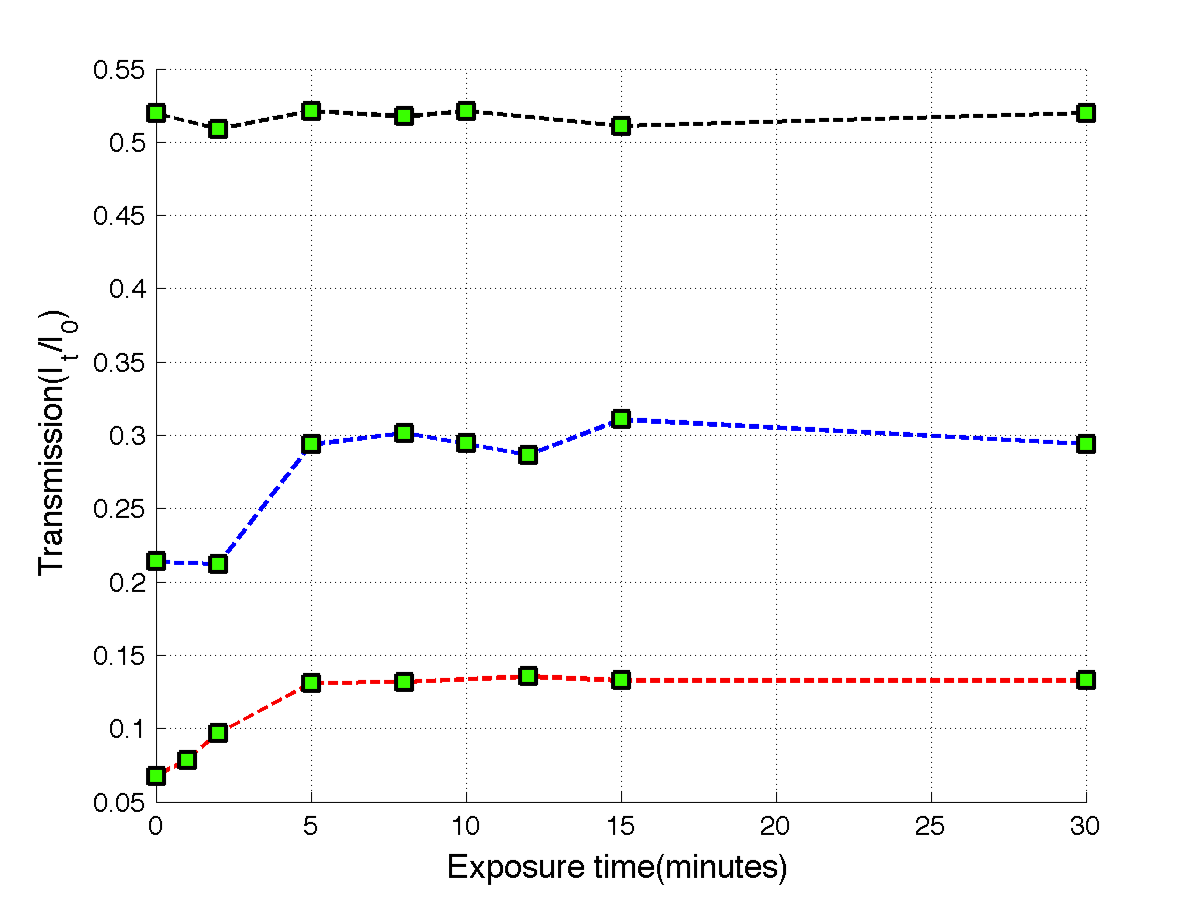
\includegraphics[width=3.25in]{figure/Transmission.png}
  \caption{Transmission study of Ag-doped As$_2$S$_3$ film, exposed to
    $\lambda = 532nm$ green laser light.
    (I$_0 \approx 10$mW; Film thickness: $1.54-2.42 \mu m$).
}
  \label{fig:setup}
\end{figure}

\begin{figure}[!h]
  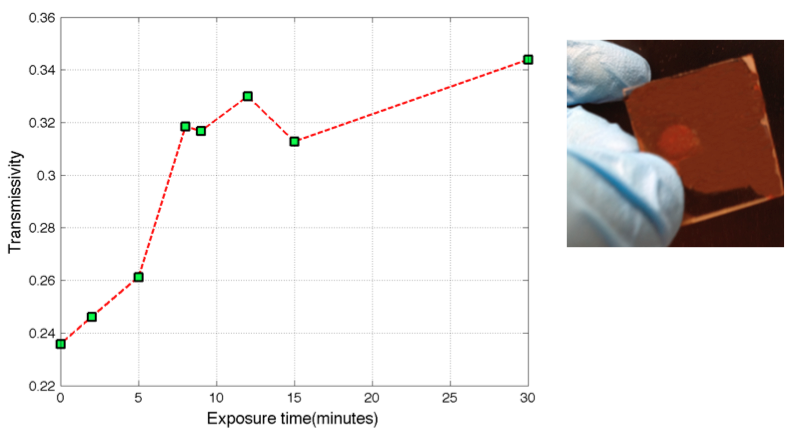
\includegraphics[width=3.25in]{figure/Transmission20nm.png}
  \caption{Transmission study of Ag($20$nm) doped As$_2$S$_3$ film, exposed to
    $\lambda = 532nm$ green laser light.
    (I$_0 \approx 10$mW).}
  \label{fig:setup}
\end{figure}


\section{Results and Discussion}
\cite{example}
\section{Conclusions}
\bibliography{references}
\end{document}

